%%%%%%%%%%%%%%%%%%%%%%%%%%%%%%%%%%
% Felix Hoffmann, October 2014
% adapted from Jyotika Bahuguna October 2012
%%%%%%%%%%%%%%%%%%%%%%%%%%%%%%%%%%


%\documentclass{beamer}
\documentclass[xcolor=table,10pt]{beamer}
\usepackage{latexsym,amssymb,amsfonts,amsmath}
\usepackage{graphicx}
\usepackage{caption}
\usepackage{minted}

%for Introduction - Part 1 - ... Orientation
%\useoutertheme[subsection=false, shadow]{miniframes} 
\useinnertheme{default}
\beamertemplatenavigationsymbolsempty

\usefonttheme{serif}
\usepackage{palatino}
\usepackage{eulervm} %additional math 


% Other Palatino font packages, with math
% see also http://tex.stackexchange.com/questions/89610
% and math_fonts.pdf in Latex docs
% --------------------
% \usepackage{pxfonts}
% \usepackage{mathpazo} % add possibly `sc` and `osf` options
% --------------------

\setbeamercolor*{structure}{fg=black}

\usepackage{transparent} % transparent graphics


\usepackage{subcaption}
\graphicspath{{img/}{../}}

\usepackage[table]{xcolor}
\usepackage{tikz}
\usetikzlibrary{arrows,shapes}
\usepackage{color}


\newminted[mlinepython]{python}{fontsize=\small, linenos,
               		numbersep=9pt,
               		gobble=4,
               		frame=lines,
                        bgcolor=bg,
               		framesep=3mm}    



\usepackage[english]{babel}
\usepackage[latin1]{inputenc}



\title {File operations, data parsing and batch files}
%\subtitle{}

\author[Felix Hoffmann]{Felix Hoffmann} 
\institute[BCF]{Bernstein Center Freiburg}
\date{\today}


\AtBeginSection[]
{
\begin {frame}<beamer>
\frametitle{}
\tableofcontents[currentsection]
\end{frame}
}


%%%%%%%%%%%%%%%%%%%%%%%%%%%%%%%%%%%%%%%%%%%%%%

\begin{document}

\begin{frame} 
  \titlepage
\end{frame}


\begin{frame} 
  \frametitle{Outline}
  \tableofcontents[pausesections]
\end{frame}

%%%%%%%%%%%%% What are they? %%%%%%%%%%% 

\section{Introduction}
\begin{frame}
\frametitle{Where do they fit?}
\begin{columns}
\column{2.0in}
\begin{itemize}
\item Data has to be read/written from/to files before/after processing    
\item Raw data needs some pre-processing.  
\item Batch files are meta scripts that automate these tasks  
\end{itemize}
\column{2.0in}
\begin{figure}
    \centering
    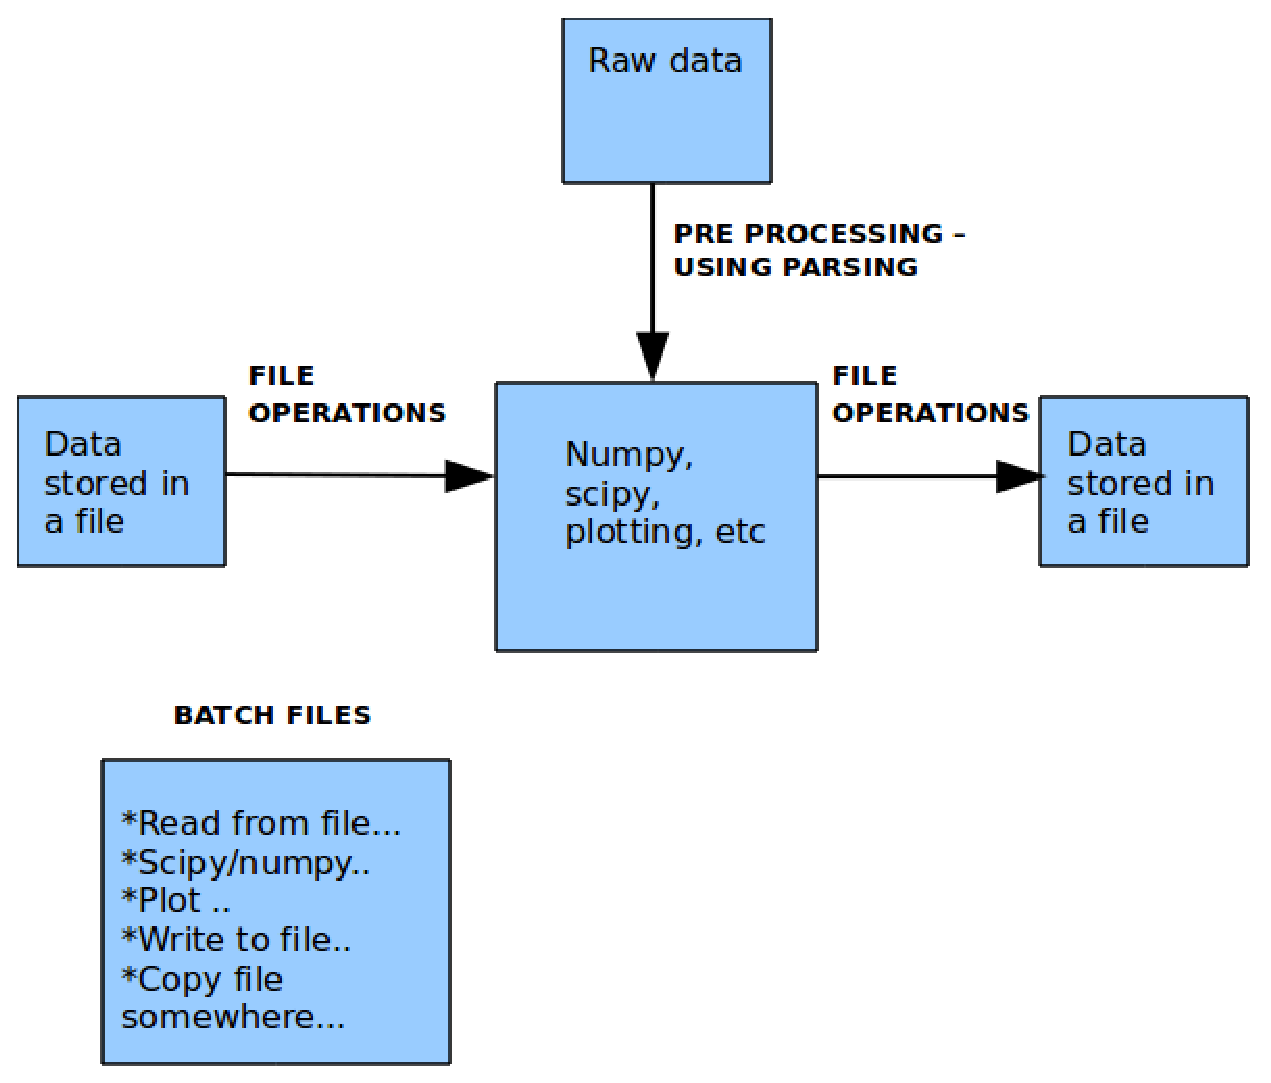
\includegraphics[width=2.0in]{Fits.eps}
\end{figure}
\end{columns}
\end{frame}

%%%%%%%%%%%%%%%%%%%%%%%%%%%%%%%%%%%%%%%%


\section{Load/Save data}



\begin{frame}[fragile]
  \frametitle{File operations}

  \begin{mlinepython}
    f = open("test.txt","r") # open test.txt in read mode
    x = f.readline() # Read one line from the file. 
    print x # This prints '21\\n'
    y = int(x)*2 # Cast x into int and multiply by 2
    f1 = open("test1.txt","w") # Open test1.txt in write mode
    f1.write(str(y)) # Note f1.write(y) will give an error
    f1.close()
    f.close()
  \end{mlinepython}

  Alternatively,

  \begin{minted}{python}
    f = open("test.txt","ra+") # open test.txt in read/append mode
    x = f.read() # Read the whole file at once.
    print x # This prints '42\\n'
    y = int(x)*2 # Cast x into int and multiply by 2
    f.write(str(y)) # Append the result to existing file 
    f.close()
  \end{minted}

  Note: The data read from the file should be casted to int/float for arithmetic operations
\end{frame}

% %%%%%%%%%%%%%%%%%%%%
% \begin{frame}[fragile]
% \frametitle{Pickle module}
% \begin{itemize}
% \item To save more complex data types - lists, dictonaries and even class objects.     
% \item Can convert any python object to string (pickling) and back(unpickling)  
% \item No cast required. 
% \end{itemize}
% \tiny
% \vspace{1mm}
% \begin{minted}{python}
% import pickle 
% x = numpy.arange(0,1,0.1)
% pickle.dump(x,open("example","w"))
% #####################
% getx = pickle.load(open("example","r"))\\
% pylab.plot(getx) 
% \end{minted}

% \end{frame}

% %%%%%%%%%%%%%%%%%%%%

% \section{Data parsing}
% \begin{frame}
% \frametitle{Need for parsing}
% \begin{columns}
% \column{2.0in}
% \begin{itemize}
% \item Data files are generated by a third party (no control over the format)
% \item Data files need pre-processing.
% \item Regular expressions provide a powerful and concise way to perform pattern match/search/replace over the data. 
% \end{itemize}
% \column{2.0in}
% \begin{figure}
%     \centering
%     
\includegraphics[width=2.0in]{regex.eps}
% \caption{\tiny{picture courtesy- www.xkcd.com} }
% \end{figure}
% \end{columns}
% \end{frame}

% % Kravitz paper here
% %%%%%%%%%%%%%%%%%%%%
% \begin{frame}
% \frametitle{Regex}
% \begin{itemize}
% \item Main challenge is to come up with a pattern using regex literals, that match the requirements of parsing.
% \item Regex literals
% 	\begin{itemize}
% 		\item \^ - Matches beginning of line/pattern
% 		\item \$ - Matches end of line/pattern
% 		\item . - Matches any character except newline
% 		\item {[}..{]} - Matches any single character in brackets
% 		\item {[}\^..{]}- Matches any single character not in brackets
% 		\item re* - Matches 0 or more occurrences of the preceding expression
% 		\item re+ - Matches 1 or more occurrences of the preceding expression
% 		\item re? - Matches 0 or 1 occurrence
% 		\item re\{n\} - Match exactly n occurrences
% 		\item re\{n,\} - Match n or more occurrences
% 		\item re\{n,m\} - Match at least n and at most m
%    	\end{itemize}
% \end{itemize}
% \end{frame}

% %%%%%%%%%%%%%%%%%%%%
% \begin{frame}[fragile]
% \frametitle{Regex - re.search()}
% \begin{itemize}
% \item Suppose the pattern to match is "python"
% \item regex module in python is "re"
% \item re.search(pattern, string, flags=0) $\rightarrow$ matches the pattern in string\\
% \tiny
% \begin{minted}{python}
% import re
% data = "I like python"
% ans = re.search(r'python',data)
% ans.group() # returns the entire match
% Out[20]: 'python'
% \end{minted}
% \small
% \item Suppose the pattern to match is "python" or "Python"\\
% \tiny
% \begin{minted}{python}
% data = "Python is a programming language. I like python"
% ans = re.search(r'[pP]ython',data)
% ans.group()
% Out[38]: 'Python'
% \end{minted}
% \small
% \item Though the regex is correct, re.search() returns as soon as it finds one instance.{[} re.findall() {]}
% \item re.match((pattern, string, flags=0), same as search() but only at start of the string 
% \end{itemize}
% \end{frame}



% %%%%%%%%%%%%%%%%%%%%
% \begin{frame}[fragile]
% \frametitle{Regex - re.findall()}
% \begin{itemize}
% \item re.findall(pattern, string, flags=0) $\rightarrow$ returns a list of all occurences of pattern\\
% \tiny
% \begin{minted}{python}
% data = "Python is a programming language. I like python"
% ans = re.findall(r'[pP]ython',data)
% print ans
% ['Python', 'python']
% \end{minted}
% \small
% \item Suppose the aim is to extract all numbers from a data stream
% \tiny
% \begin{minted}{python}
% data = "There are 7 students and 2 tutors"\\
% ans = re.findall(r'[0-9]+',data)\\
% print ans
% ['7', '2']
% \end{minted}
% \small
% (Note these are strings and need to be cast into integers for arthimetic operation)\\
% \end{itemize}
% \end{frame}



% %%%%%%%%%%%%%%%%%%%%
% \begin{frame}[fragile]
% \frametitle{Regex - More examples}
% \begin{itemize}
% \item Suppose the aim is to extract strings not numbers
% \tiny
% \begin{minted}{python}
% data = "There are 7 students and 2 tutors"
% ans = re.findall(r'[^ 0-9]+',data)
% print ans
% ['There are ', ' students and ', ' tutors']
% \end{minted}
% \small
% \item Multiple regular expressions can be used to perform the job. For eg,\\
% \tiny
% \begin{minted}{python}
% ans = re.findall(r'[a-zA-Z]+',data)
% print ans
% ['There', 'are', 'students', 'and', 'tutors']
% \end{minted}
% \small
% \item However slight difference. 
% \end{itemize}
% \end{frame}

% %%%%%%%%%%%%%%%%%%%%
% \begin{frame}[fragile]
% \frametitle{Regex -  re.split()}
% \begin{itemize}
% \item Suppose the data stream has well-defined delimiter.\\
% \tiny
% \begin{minted}{python}
% data = "x = 20"
% ans = re.split(r'=',data)
% print ans
% ['x', '20']
% \end{minted}
% \vspace{1mm}
% \begin{minted}{python} 
% data = 'ftp://python.about.com'
% ans = re.split(':/{1,3}', data)
% print ans
% ['ftp', 'python.about.com']
% \end{minted}
% \small
% \item Searching for regex literals as strings. Escape the meaning by a preceding backslash $\backslash$
% \tiny
% \begin{minted}{python}
% data = '25.657' # Split into whole and fractional parts
% ans = re.split(r'\.',data)
% print ans
% ['25', '657']
% \end{minted}
% \end{itemize}
% \end{frame}

% %%%%%%%%%%%%%%%%%%%%
% \begin{frame}[fragile]
% \frametitle{Regex -  re.sub()}
% \begin{itemize}
% \item Most powerful of them all.
% \item re.sub(pattern, repl, string, max=0) looks for a pattern and replaces with repl
% \item Aim is to delete python style comments in the line below:\\
% \tiny
% \begin{minted}{python}
% data = "2004-959-559 #This is Phone Number"
% ans = re.sub(r'#.*','',data)
% print ans
% '2004-959-559 '
% \end{minted}
% \small
% \item Now delete the hyphens from the above phone number.\\
% \tiny
% \begin{minted}{python}
% ans1 = re.sub(r'-','',ans)
% print ans1
% '2004959559 '
% \end{minted}
% \end{itemize}
% \end{frame}

% %%%%%%%%%%%%%%%%%%%%
% \begin{frame}
% \frametitle{Regex - Some shortcuts}
% \begin{itemize}
% \item $\backslash$w - Matches word character 
% \item $\backslash$W - Matches non-word character
% \item $\backslash$s - Matches whitespace (Equivalent to $\backslash$t$\backslash$n$\backslash$r," ")
% \item $\backslash$S - Matches non-whitespace.
% \item $\backslash$d - Matches digits (Equivalent to {[}0-9{]} )
% \item $\backslash$D - Matches non digits
% \item $\backslash$A - Matches beginning of the string
% \item $\backslash$Z - Matches end of the string
% \item $\backslash$B - Matches nonword boundaries
% \item $\backslash$n,$\backslash$t - Matches newline, tab resp
% \end{itemize}
% \end{frame}

% %%%%%%%%%%%%%%%%%%%%


% %%%%%%%%%%%%% What are they? %%%%%%%%%%% 
% \section{Batch files}
% %%%%%%%%%%%%%%%%%%%%%%%%%%%%%%%%%%%%%%%%
% %%%%%%%%%%%%%%%%%%%%
% \begin{frame}[fragile]
% \frametitle{os module}
% \begin{itemize}
% \item Meta scripts that can automate your task
% \item os module in python provides a way of using os dependent functionality
% 	\begin{itemize}
% 	\item os.mkdir() - Creates a directory (like mkdir)
% 	\item os.chmod() - Change the permissions (like chmod)
% 	\item os.rename() - Rename the old file name with the new file name.\	
% 	\item os.listdir() - List the contents of the directory\
% 	\end{itemize}
% \item batch file batch\_file.py to run your script exercise.py for all data files in a directory.\\
% \tiny
% \begin{minted}{python}
% from os import listdir
% files = listdir(".")
% for f in files: 
% 	os.system('python exercise.py f')
% \end{minted}
% \end{itemize}
% \end{frame}

% %%%%%%%%%%%%%%%%%%%%
% \begin{frame}
% \frametitle{Summary}
% \begin{itemize}
% \item Using these libraries, a lot of workflow can be automated.
% \item One doesnt require to learn something separate for pre-processing, processing and automation. Python does it all.
% \end{itemize}

% Suggestion for exercises:
% Test your regex on the file "regextest.gdf" first.\\ It is a reduced version of data files(only 100 data points).\\
% Hence visual inspection can be used easily to check if regex worked correctly.
% \end{frame} 




\end{document}

